\documentclass[leqno]{article}
% Shared QBT/Soln pack preamble for resources.danieljsmith.org.
\usepackage{graphicx}
\usepackage{dsfont}
\usepackage{mathtools}
\usepackage{amssymb}
\usepackage{amsmath}
\usepackage{mleftright}
\usepackage{amsthm}
\usepackage{float}
\usepackage{ragged2e}
\usepackage{tensor}
\usepackage{fancyhdr}
\usepackage{empheq}
\usepackage[most]{tcolorbox}
\usepackage{enumitem}
\usepackage{dirtytalk}
\usepackage{marginnote}
\usepackage{microtype}
\usepackage[
  a4paper,
  left=0.8in,
  right=1in,
  top=1in,
  bottom=0.5in,
  headheight=14pt,
  headsep=0.4in
]{geometry}
\setlength{\parindent}{0cm}

% TikZ / PGFPlots
\usepackage{pgfplots}
\pgfplotsset{compat=1.18}
\usepgfplotslibrary{fillbetween, polar}
\usetikzlibrary{calc, positioning}
\usetikzlibrary{angles, quotes}
\usetikzlibrary{arrows.meta}
\usetikzlibrary{decorations.pathreplacing, decorations.markings}
\usetikzlibrary{patterns}
\usetikzlibrary{intersections}

% Links and contents. The contents follow the TMUA papers: compact entries,
% no dot leaders, and each question's mark total in grey after its label.
\usepackage{tocloft}
\tocloftpagestyle{fancy}
\setlength{\cftbeforesubsecskip}{2pt}
\setlength{\cftsubsecindent}{1.5em}
\setlength{\cftsubsecnumwidth}{0pt}
\renewcommand{\cftsubsecfont}{\small\color{black}}
\renewcommand{\cftsubsecpagefont}{\small\color{black}}
\renewcommand{\cftsubsecleader}{\hfill}
\usepackage[colorlinks=true,linkcolor=black,citecolor=magenta,urlcolor=black]{hyperref}%
\urlstyle{same}

% Pack macros
% \marks also adds its value to the current question's total in the .aux
% file, so the contents show each total from the second pass. The write
% happens at shipout, so a box typeset more than once counts once. The
% pack's mark total for the contents-page title is summed the same way.
\makeatletter
\newcount\djs@totalmarks
\newcommand{\djsAddMarks}[2]{%
  \global\advance\djs@totalmarks#2\relax
  \@ifundefined{djs@marks@#1}%
    {\expandafter\xdef\csname djs@marks@#1\endcsname{#2}}%
    {\expandafter\xdef\csname djs@marks@#1\endcsname
      {\the\numexpr\csname djs@marks@#1\endcsname+#2\relax}}}
\RenewDocumentCommand{\marks}{o m}{%
  \protected@write\@auxout{}{\string\djsAddMarks{\number\value{enumi}}{#2}}%
  \IfValueTF{#1}%
    {\marginnote{\raggedright\textbf{[#2]}}[#1]}%
    {\marginnote{\raggedright\textbf{[#2]}}}%
}
\makeatother

\newcommand{\vspacerule}[2]{%
  \par\vspace*{#1}%
  \noindent\hrulefill\par
  \vspace*{#2}%
}

\definecolor{scarlet}{RGB}{205, 40, 75}
% Site colours for the contents-page title: the accent, the rule colour, a
% stronger rule colour for the path separator, and the muted text colour.
\definecolor{djsBurgundy}{RGB}{118, 59, 67}
\definecolor{djsHairline}{RGB}{216, 213, 205}
\definecolor{djsSlash}{RGB}{170, 166, 158}
\definecolor{djsMuted}{RGB}{96, 101, 106}

% Worked-solution box, adapted from the TMUA worked-solutions box. A white breakable box with a left scarlet rule and no surrounding
% frame or tint. A part that breaks fills the rest of its page, so the rule
% runs to the bottom margin; the unbroken or last part ends in a short
% horizontal foot rule so a solution visibly stops. Unlike the TMUA box there
% is no answer label. The box does not grow to the left, so the rule sits at
% the text edge; growing to the right keeps the usable line width close to the
% old tcolorbox Solution box.
% Spacing inside the box: paragraphs are 6pt apart, so source blank lines show
% (solutions put one after each display and none between a lead-in and its
% display). Every display gets 6pt above and 10pt below, whatever the length
% of its lead-in line; align rows are spread by an 8pt \jot; solution parts
% are 14pt apart and sub-parts 8pt; \left and \right space like ordinary
% brackets (mleftright); no single line is stranded at a page break; and
% neither the Solution label nor the line before a list ends a page. No
% skip can shrink, so full pages are not squeezed.
\newtcolorbox{djsSolution}{%
  enhanced, breakable, frame hidden, sharp corners, colback=white,
  height fixed for=first and middle, height fill,
  extras unbroken and last={natural height},
  borderline west={2.2pt}{0pt}{scarlet},
  left=11pt, right=0pt, top=5pt, bottom=13pt,
  before skip=13pt, after skip=4pt,
  grow to right by=10mm,
  overlay unbroken and last={%
    \fill[scarlet] (frame.south west)
      rectangle ([xshift=3.5cm, yshift=2.2pt]frame.south west);},
  before upper={{\color{scarlet}\bfseries Solution}\par\nobreak\vspace{4pt}%
    \setlength{\parskip}{6pt plus 2pt}%
    \setlength{\abovedisplayskip}{6pt plus 2pt}%
    \setlength{\abovedisplayshortskip}{6pt plus 2pt}%
    \setlength{\belowdisplayskip}{10pt plus 2pt}%
    \setlength{\belowdisplayshortskip}{10pt plus 2pt}%
    \setlength{\jot}{8pt}%
    \setlist{parsep=6pt plus 2pt, topsep=6pt plus 2pt, beginpenalty=10000}%
    \setlist[enumerate,1]{itemsep=14pt plus 2pt}%
    \setlist[enumerate,2]{itemsep=8pt plus 2pt}%
    \mleftright
    \clubpenalty=10000 \widowpenalty=10000 \displaywidowpenalty=10000\relax}}

% Optional smaller figure inside a solution box. \scalebox shrinks node text
% with the drawing. Not applied to existing figures.
\newcommand{\SolnFigureScale}{0.85}
\newsavebox{\djsSolnFigureBox}
\newenvironment{djsSolutionFigure}
  {\par\vspace{4pt}\begin{center}\begin{lrbox}{\djsSolnFigureBox}}
  {\end{lrbox}\scalebox{\SolnFigureScale}{\usebox{\djsSolnFigureBox}}%
   \end{center}\vspace{2pt}\par}

\newcommand{\cxl}[2]{%
  \tikz[baseline=(X.base)]{%
    \node[inner sep=0pt, outer sep=0pt, text=#1] (X) {$#2$};
    \draw[#1, line width=0.4pt] (X.south west)--(X.north east);
  }%
}

% Page-style hook run at the contents page and each question's opening page.
% A no-op for QBT packs; \djsSolnHeader points it at the fancy header.
\newcommand{\djsQuestionPageStyle}{}

% A contents entry: "Question N" in a box wide enough for two digits, so the
% mark totals line up, then the total in grey. Bookmarks keep "Question N".
\makeatletter
\newlength{\djsTocLabelWidth}
\newcommand{\djsTocMarks}[1]{%
  \@ifundefined{djs@marks@#1}{}{%
    {\footnotesize\itshape\color{black!45}%
     \csname djs@marks@#1\endcsname~mark%
     \ifnum\csname djs@marks@#1\endcsname=1 \else s\fi}}}
\newcommand{\djsTocEntry}[1]{%
  \texorpdfstring
    {\settowidth{\djsTocLabelWidth}{Question 00}%
     \makebox[\dimexpr\djsTocLabelWidth+0.9em\relax][l]{Question #1}%
     \djsTocMarks{#1}}%
    {Question #1}}
\makeatother

% The question count for the contents-page title is written to the .aux at
% the end of the document, so it also appears from the second pass.
\newcounter{djsQuestions}
\newcommand{\questionitem}{%
  \djsQuestionPageStyle
  \item\phantomsection
  \stepcounter{djsQuestions}%
  \addcontentsline{toc}{subsection}{\protect\djsTocEntry{\number\value{enumi}}}%
}
\makeatletter
\newcommand{\djsSetQuestionCount}[1]{\gdef\djs@questioncount{#1}}
\AtEndDocument{\immediate\write\@auxout
  {\string\djsSetQuestionCount{\number\value{djsQuestions}}}}
\makeatother

\renewcommand{\contentsname}{Questions}

% \djsPackHeader[<link content tag>]{<left header>}; the tag says which
% document a click on the header link came from.
\newcommand{\djsPackHeader}[2][questions]{%
  \pagestyle{fancy}%
  \fancyhead{}%
  \fancyfoot{}%
  \renewcommand{\headrulewidth}{0.9pt}%
  \lhead{#2}%
  \chead{}%
  \rhead{\href{https://danieljsmith.org/?utm_source=pdf&utm_campaign=further-maths&utm_content=#1}{danieljsmith.org}}%
}

% The header's topic is also the contents-page title, under which a label
% says which booklet this is.
\newcommand{\djsPackTitle}{}
\newcommand{\djsBookletLabel}{}
\newcommand{\djsQbtHeader}[1]{%
  \djsPackHeader{#1}%
  \renewcommand{\djsPackTitle}{#1}%
  \renewcommand{\djsBookletLabel}{Questions by topic}%
}

% The colophon at the foot of page one, independent of the page style: the
% contents-page title's hairline led by a short scarlet rule, then the date on
% the left and a link to the site on the right, all inside the bottom margin.
% Its sizes are fixed, so it matches the TMUA papers' colophon. The document
% supplies the date; recompiling never changes it.
\makeatletter
\newcommand{\djsLastUpdated}[1]{%
  \AtBeginDocument{\AddToHookNext{shipout/foreground}{\djs@colophon{#1}}}}
\newcommand{\djs@colophon}[1]{%
  \put(0.8in,-\dimexpr\paperheight-0.47in\relax){%
    \makebox[0pt][l]{\color{djsHairline}%
      \rule[0.9pt]{\dimexpr\paperwidth-1.8in\relax}{0.6pt}}%
    \makebox[0pt][l]{\color{scarlet}\rule{3.5cm}{2.2pt}}}%
  \put(0.8in,-\dimexpr\paperheight-0.32in\relax){\makebox[0pt][l]{%
    \fontsize{9}{11}\selectfont Last updated #1}}%
  \put(\dimexpr\paperwidth-1in\relax,-\dimexpr\paperheight-0.32in\relax){%
    \makebox[0pt][r]{\fontsize{7}{8.5}\selectfont\color{djsMuted}%
      Latest version at \href{https://resources.danieljsmith.org/}%
        {\color{black}resources.danieljsmith.org}}}}
\makeatother

% Solutions packs show the header only on the contents page and each
% question's opening page, so it never appears part-way through a solution.
% \thispagestyle marks the next page shipped out, which is the question's
% page because every solution question starts after a \newpage.
\newcommand{\djsSolnHeader}[1]{%
  \djsPackHeader[solutions]{\textit{Solutions} - #1}%
  \pagestyle{empty}%
  \renewcommand{\djsQuestionPageStyle}{\thispagestyle{fancy}}%
  \renewcommand{\djsPackTitle}{#1}%
  \renewcommand{\djsBookletLabel}{Worked solutions}%
}

% \djsSitePath{<strand>}{<topic>}, called once after the header, names where
% the pack sits on the site; the contents-page title prints it above the pack
% title, e.g. CORE PURE / FURTHER CALCULUS. Without it the line is left out.
\makeatletter
\newif\ifdjs@sitepath
\newcommand{\djs@strand}{}
\newcommand{\djs@section}{}
\newcommand{\djsSitePath}[2]{%
  \djs@sitepathtrue
  \renewcommand{\djs@strand}{#1}%
  \renewcommand{\djs@section}{#2}%
}
\makeatother

% Further Mechanics packs call \djsMechanicsPack in their preamble, so that
% \djsFrontMatter prints the default value of g above the contents. The box
% keeps its own space above it (before skip is the whole gap below the title,
% not an addition to it). Without the box, \djsGravityNote is just extra space
% before the contents heading, bringing the gap above it close to the gap
% between the box and the heading on Further Mechanics pages.
\newcommand{\djsGravityNote}{\vspace{14pt}}
\newcommand{\djsMechanicsPack}{%
  \renewcommand{\djsGravityNote}{%
    \begin{tcolorbox}[sharp corners, colback=white, colframe=black,
      boxrule=1pt, left=8pt, right=8pt, top=6pt, bottom=6pt,
      before skip=20pt]
    {\bfseries Instructions}\par\vspace{4pt}
    Unless a question states otherwise, take $g = 9.8\,\mathrm{m\,s^{-2}}$
    wherever a numerical value of $g$ is required. Solutions also give final
    answers for $g = 10\,\mathrm{m\,s^{-2}}$ where these differ.
    \end{tcolorbox}%
    \vspace{16pt}}%
}

% Contents-page title: the site path in spaced burgundy capitals, the pack
% title, a hairline led by a short scarlet rule (the solution box's foot rule),
% then the booklet label with the question and mark counts. The counts come
% from the .aux, so they appear from the second pass.
\makeatletter
\newsavebox{\djs@eyebrowbox}
\newcommand{\djs@caps}[1]{\textls[180]{\MakeUppercase{#1}}}
\newcommand{\djs@eyebrow}{%
  \color{djsBurgundy}\footnotesize\bfseries
  \djs@caps{\djs@strand}%
  {\color{djsSlash}\hspace{0.55em}/\hspace{0.55em}}%
  \djs@caps{\djs@section}}
\newcommand{\djs@dot}{\hspace{0.45em}\textperiodcentered\hspace{0.45em}}
\newcommand{\djs@counts}{%
  \@ifundefined{djs@questioncount}{}{%
    \djs@questioncount~question\ifnum\djs@questioncount=1 \else s\fi
    \ifnum\djs@totalmarks>0
      \djs@dot\the\djs@totalmarks~mark\ifnum\djs@totalmarks=1 \else s\fi
    \fi}}
\newcommand{\djsContentsTitle}{%
  \ifdjs@sitepath
    \sbox\djs@eyebrowbox{\djs@eyebrow}%
    \ifdim\wd\djs@eyebrowbox>\linewidth
      \@latex@warning@no@line{The \string\djsSitePath\space line is wider
        than the text, so it wraps. Shorten its topic}%
    \fi
    {\raggedright\djs@eyebrow\par}%
    \vspace{7pt}%
  \fi
  {\raggedright\fontsize{24.88}{28}\selectfont\djsPackTitle\par}%
  \vspace{9pt}%
  \noindent\makebox[0pt][l]{\color{djsHairline}\rule[0.9pt]{\linewidth}{0.6pt}}%
  {\color{scarlet}\rule{3.5cm}{2.2pt}}\par
  \vspace{5pt}%
  {\small\color{djsMuted}\djsBookletLabel\hfill\djs@counts\par}%
  \vspace{8pt}%
}
\makeatother

\newcommand{\djsFrontMatter}{%
  \djsQuestionPageStyle
  \vspace*{6pt}%
  \djsContentsTitle
  \djsGravityNote
  \tableofcontents
  \newpage
}


\djsQbtHeader{Projectile Motion}
\djsSitePath{Further Mechanics}{Kinematics \& Dynamics}
\djsMechanicsPack
\djsLastUpdated{15 October 2026}

\begin{document}
\djsFrontMatter
\begin{enumerate}[
  label=\textbf{\arabic*.},
  leftmargin=*,
  topsep=0pt,
  partopsep=0pt,
  parsep=0pt
]

% ---- Question 1 ----
\questionitem
% [Source: _QBT__Projectile_Motion, Q1]

A particle $P$ is projected from a point $O$ at the edge of a cliff, $40\,\mathrm{m}$ above horizontal ground. \\
Its initial speed is $u\,\mathrm{m\,s^{-1}}$ and its angle of projection is $30^\circ$ above the horizontal, directed away from the cliff. \\
The particle moves freely under gravity until it strikes the ground. \\

Immediately before impact, the direction of motion of $P$ is perpendicular to its initial direction of motion. \\

Find the initial speed $u$ and the time taken to reach the ground, giving both answers in exact form. \marks{8} \\

\newpage

% ---- Question 2 ----
\questionitem
% [Source: _QBT__Projectile_Motion, Q2]

A particle $P$ is projected from a point $O$, which is $30\,\mathrm{m}$ above horizontal ground, with speed $u\,\mathrm{m\,s^{-1}}$ at an angle $\theta$ above the horizontal, where $0<\theta<90^\circ$. \\
The particle moves freely under gravity and lands on the ground at a horizontal distance of $40\,\mathrm{m}$ from $O$. \\

The velocity of $P$ immediately before it lands is perpendicular to its initial velocity. \\

Find $u$ and $\theta$, giving the angle to one decimal place. \marks{8} \\

\newpage

% ---- Question 3 ----
\questionitem
% [Source: _QBT__Projectile_Motion, Q3]

A particle $P$ is projected from a point $O$ at time $t=0$ with speed $u\,\mathrm{m\,s^{-1}}$ at an angle $\theta$ above the horizontal, where $0<\theta<90^\circ$. \\
The particle moves freely under gravity, with $g=10\,\mathrm{m\,s^{-2}}$. \\
After $6$ seconds, its speed is $\sqrt{5}u\,\mathrm{m\,s^{-1}}$. \\

\begin{enumerate}[label=\textbf{(\alph*)}]
\item Show that
\[
u^2+30u\sin\theta-900=0
\] \marks[-20pt]{3}
\item At time $t=6\,\mathrm{s}$, the particle is at a point $A$ below the horizontal level of $O$. \\
The displacement vector $\overrightarrow{OA}$ is perpendicular to the initial velocity of $P$. \\
Find the exact value of $u$, the value of $\theta$, and the exact distance $OA$. \marks{6} \\
\end{enumerate}

\newpage

% ---- Question 4 ----
\questionitem
% [Source: _QBT__Projectile_Motion, Q4]

At time $t=0$, a particle $P$ is projected from a point $O$ on horizontal ground with speed $26\,\mathrm{m\,s^{-1}}$ at an angle $\alpha$ above the horizontal, where $\sin\alpha=\frac{12}{13}$. \\
A point $A$ on the ground lies $40\,\mathrm{m}$ from $O$ in the direction of the horizontal motion of $P$. \\

At time $t=T\,\mathrm{s}$, where $T>0$, a second particle $Q$ is projected vertically upwards from $A$ with speed $22\,\mathrm{m\,s^{-1}}$. \\
The particles collide while $Q$ is travelling upwards. \\
Before the collision, both particles move freely under gravity. \\
Neglect air resistance throughout. \\

\begin{enumerate}[label=\textbf{(\alph*)}]
\item Find the time at which the particles collide and their height above the ground at that instant. \marks{2} \\
\item Find the exact value of $T$. \marks{5} \\
\item Immediately after the collision, the speed of $P$ is $v\,\mathrm{m\,s^{-1}}$ and its direction of motion is above the horizontal. \\
Its horizontal velocity component is unchanged by the collision, and it subsequently moves freely under gravity. \\
Find its greatest height above the ground in terms of $v$. Hence find the least possible value of $v$ for $P$ to reach a height of $40\,\mathrm{m}$ above the ground. \marks{4} \\
\end{enumerate}

\newpage

% ---- Question 5 ----
\questionitem
% [Source: _QBT__Projectile_Motion, Q5]

A particle $P$ is projected from a point $A$ which is vertically above a fixed point $O$ on horizontal ground, with $OA=h$. \\
Its initial velocity is $u(4\mathbf{i}+3\mathbf{j})$, where $u>0$ and $h>0$. \\
The unit vectors $\mathbf{i}$ and $\mathbf{j}$ are horizontal and vertically upwards respectively. \\
The particle moves freely under gravity, with constant acceleration $-g\mathbf{j}$. \\

At time $t=0$, the particle leaves $A$. \\
Its position vector relative to $O$ at time $t$ is $\mathbf{r}=x\mathbf{i}+y\mathbf{j}$. \\

\begin{enumerate}[label=\textbf{(\alph*)}]
\item Starting from an expression for $\ddot{\mathbf{r}}$, use integration to obtain $\mathbf{r}$ in terms of $t$, $u$, $h$ and $g$. \marks{4} \\
\item Eliminate $t$ to obtain the Cartesian equation of the path of $P$. \marks{3} \\
\item Hence find the maximum height of $P$ above the ground, in terms of $u$, $h$ and $g$. \marks{3} \\
\item When $P$ first strikes the ground, its velocity is perpendicular to its initial velocity. Determine $h$ in terms of $u$ and $g$. \marks{4} \\
\end{enumerate}

\newpage

% ---- Question 6 ----
\questionitem
% [Source: _QBT__Projectile_Motion, Q6]

\begin{figure}[H]
    \centering
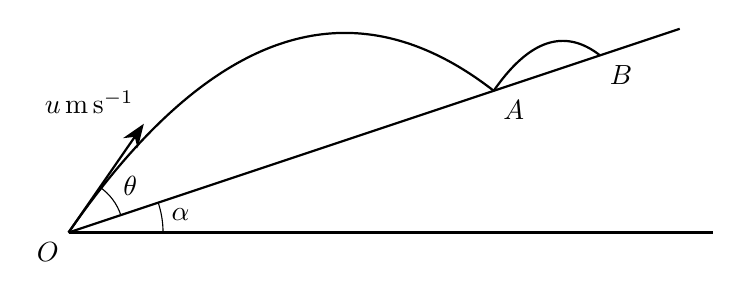
\begin{tikzpicture}[x=0.12cm,y=0.12cm]
\def\grav{10}
\def\launchSpeed{25}
\def\tanAlpha{1/3}
\def\tanTheta{3/4}
\def\restitution{0.5}
\def\arrowLength{14}
\def\extension{1.15}
\pgfmathsetmacro{\alph}{atan(\tanAlpha)}
\pgfmathsetmacro{\thet}{atan(\tanTheta)}
\pgfmathsetmacro{\gs}{\grav*sin(\alph)}
\pgfmathsetmacro{\gn}{\grav*cos(\alph)}
\pgfmathsetmacro{\us}{\launchSpeed*cos(\thet)}
\pgfmathsetmacro{\un}{\launchSpeed*sin(\thet)}
\pgfmathsetmacro{\firstTime}{2*\un/\gn}
\pgfmathsetmacro{\sA}{\us*\firstTime-\gs*\firstTime^2/2}
\pgfmathsetmacro{\vs}{\us-\gs*\firstTime}
\pgfmathsetmacro{\vn}{\restitution*\un}
\pgfmathsetmacro{\secondTime}{2*\vn/\gn}
\pgfmathsetmacro{\sB}{\sA+\vs*\secondTime-\gs*\secondTime^2/2}
\coordinate (O) at (0,0);
\coordinate (H) at ({\extension*\sB},0);
\draw[thick,black] (O) -- (H);
\begin{scope}[rotate=\alph]
  \coordinate (A) at (\sA,0);
  \coordinate (B) at (\sB,0);
  \coordinate (S) at ({\extension*\sB},0);
  \coordinate (V) at (\thet:\arrowLength);
  \draw[thick,black] (O) -- (S);
  \draw[thick,black,domain=0:\firstTime,samples=120,variable=\t]
    plot ({\us*\t-\gs*\t^2/2},{\un*\t-\gn*\t^2/2});
  \draw[thick,black,domain=0:\secondTime,samples=100,variable=\t]
    plot ({\sA+\vs*\t-\gs*\t^2/2},{\vn*\t-\gn*\t^2/2});
  \draw[-{Stealth[length=3mm]},thick,black] (O) -- (V)
    node[above left] {$u\,\mathrm{m\,s^{-1}}$};
\end{scope}
\pic["$\alpha$",draw,angle radius=12mm,angle eccentricity=1.2] {angle=H--O--S};
\pic["$\theta$",draw,angle radius=7mm,angle eccentricity=1.4] {angle=S--O--V};
\node[below left] at (O) {$O$};
\node[below right] at (A) {$A$};
\node[below right] at (B) {$B$};
\end{tikzpicture}
\end{figure}


A small ball $P$ is projected from a point $O$ at the foot of a smooth plane inclined at an angle $\alpha$ to the horizontal, where $\tan\alpha=\frac{1}{3}$. \\
Its initial speed is $u\,\mathrm{m\,s^{-1}}$, and its initial velocity makes an angle $\theta$ above the plane, where $\tan\theta=\frac{3}{4}$. \\

The ball first strikes the plane at $A$, where $OA=15\sqrt{10}\,\mathrm{m}$. \\
Its motion takes place in the vertical plane containing a line of greatest slope of the inclined plane, and air resistance is negligible. \\

\begin{enumerate}[label=\textbf{(\alph*)}]
\item Find $u$ and the components of the ball's velocity parallel and perpendicular to the plane immediately before impact at $A$. State the direction of each component. \marks{8} \\
\end{enumerate}
The ball rebounds from the plane at $A$ and next strikes it at $B$, further up the plane, where
\[
AB=\frac{15\sqrt{10}}{4}\,\mathrm{m}
\] \\
\begin{enumerate}[label=\textbf{(\alph*)}, resume]
\item Find the coefficient of restitution between the ball and the plane, explaining why any other algebraic solution must be rejected. \marks{8} \\
\end{enumerate}

\newpage

% ---- Question 7 ----
\questionitem
% [Source: _QBT__Projectile_Motion, Q7]

\begin{figure}[H]
    \centering
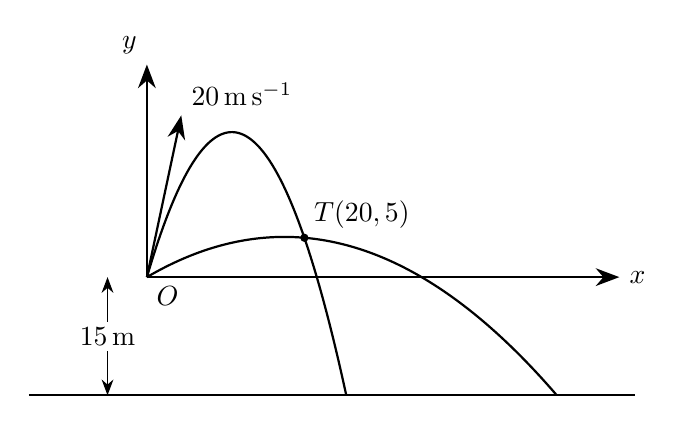
\begin{tikzpicture}[x=0.10cm,y=0.10cm]
\def\speed{20}
\def\grav{10}
\def\height{15}
\def\targetX{20}
\def\targetY{5}
\def\groundLeft{-15}
\def\groundRight{62}
\def\axisRight{60}
\def\axisTop{27}
\def\arrowAngle{78}
\def\arrowLength{21}
\def\dimOffset{5}
\pgfmathsetmacro{\lowAngle}{atan(2-sqrt(2))}
\pgfmathsetmacro{\highAngle}{atan(2+sqrt(2))}
\coordinate (O) at (0,0);
\coordinate (G) at (0,-\height);
\coordinate (T) at (\targetX,\targetY);
\coordinate (Dtop) at ($(O)+(-\dimOffset,0)$);
\coordinate (Dbottom) at ($(G)+(-\dimOffset,0)$);
\draw[thick,black] (\groundLeft,-\height) -- (\groundRight,-\height);
\foreach \ang in {\highAngle,\lowAngle} {
  \pgfmathsetmacro{\flight}{(\speed*sin(\ang)+sqrt((\speed*sin(\ang))^2+2*\grav*\height))/\grav}
  \draw[thick,black,domain=0:\flight,samples=120,variable=\t] plot ({\speed*cos(\ang)*\t},{\speed*sin(\ang)*\t-\grav*\t^2/2});
}
\draw[-{Stealth[length=3mm]},thick,black] (O) -- (\axisRight,0) node[right] {$x$};
\draw[-{Stealth[length=3mm]},thick,black] (O) -- (0,\axisTop) node[above left] {$y$};
\draw[-{Stealth[length=3mm]},thick,black] (O) -- ++(\arrowAngle:\arrowLength) node[above right] {$20\,\mathrm{m\,s^{-1}}$};
\draw[{Stealth[length=2mm]}-{Stealth[length=2mm]}] (Dbottom) -- (Dtop) node[midway,fill=white,inner sep=2pt] {$15\,\mathrm{m}$};
\fill[black] (T) circle (1.5pt);
\node[above right] at (T) {$T(20,5)$};
\node[below right] at (O) {$O$};
\end{tikzpicture}
\end{figure}


A launcher projects balls at speed $20\,\mathrm{m\,s^{-1}}$ from a point $O$, which is $15\,\mathrm{m}$ above horizontal ground. \\
Horizontal and vertically upwards displacements from $O$ are denoted by $x\,\mathrm{m}$ and $y\,\mathrm{m}$ respectively. \\
A small target $T$ has coordinates $(20,5)$, as shown in the diagram above. \\

At time $t=0$, a ball $B$ is projected at an angle $\theta$ above the positive horizontal direction, where $0\leq\theta<90^\circ$. \\
Model the ball as a particle moving freely under gravity until it first reaches the ground. \\

\begin{enumerate}[label=\textbf{(\alph*)}]
\item By first writing $x$ and $y$ in terms of $t$, find the two possible values of $\theta$ for which the ball passes through $T$. Give the angles to the nearest $0.1^\circ$. \marks{5} \\
\item For a fixed horizontal displacement $x>0$, use a quadratic in $\tan\theta$ to determine the greatest height $y$ that the ball can reach. Hence state the equation of the upper boundary of the reachable region to the right of the $y$-axis. \marks{3} \\
\item Hence find the greatest possible horizontal distance from $O$ to the point where the ball first reaches the ground, giving your answer exactly. Find also the launch angle that achieves this distance, to the nearest $0.1^\circ$. \marks{3} \\
\end{enumerate}

\newpage

% ---- Question 8 ----
\questionitem
% [Source: _QBT__Projectile_Motion, Q8]

A plane is inclined at an unknown angle $\alpha$ above the horizontal, where $0<\alpha<90^\circ$. \\
Points $O$ and $A$ lie on a line of greatest slope of the plane, with $A$ uphill from $O$ and $OA=18\,\mathrm{m}$. \\

A particle is projected from $O$ with speed $u\,\mathrm{m\,s^{-1}}$ at an angle $\theta$ above the horizontal, where $\tan\theta=3$ and $0<\theta<90^\circ$. \\
Its initial horizontal velocity is directed towards $A$. \\
The particle moves freely under gravity in the vertical plane containing $O$ and $A$. \\

The particle strikes the inclined plane at $A$, and its velocity immediately before impact is perpendicular to the inclined plane. \\

Find all possible pairs of values of $\alpha$ and $u$, giving each value to 3 significant figures. \marks{7} \\

\newpage

% ---- Question 9 ----
\questionitem
% [Source: _QBT__Projectile_Motion, Q9]

\begin{figure}[H]
    \centering
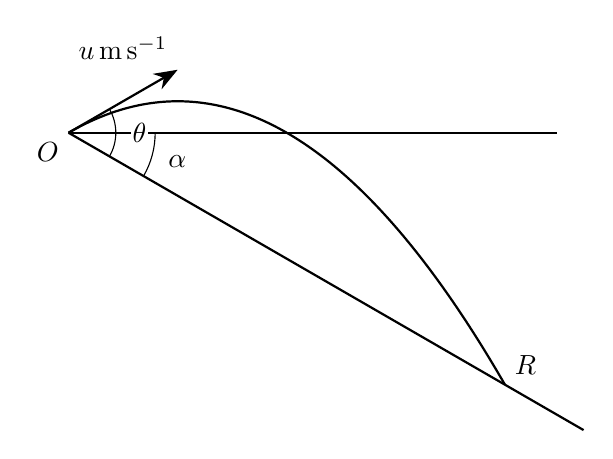
\begin{tikzpicture}[scale=0.32]
\def\incline{30}
\def\launchAngle{60}
\def\speed{10}
\def\grav{10}
\def\planeExtension{1.18}
\def\horizontalExtension{1.12}
\def\velocityLength{5}
\pgfmathsetmacro{\elevation}{\launchAngle-\incline}
\pgfmathsetmacro{\flightTime}{2*\speed*sin(\launchAngle)/(\grav*cos(\incline))}
\pgfmathsetmacro{\xR}{\speed*cos(\elevation)*\flightTime}
\pgfmathsetmacro{\yR}{-\xR*tan(\incline)}
\pgfmathsetmacro{\quadCoeff}{\grav/(2*\speed^2*cos(\elevation)^2)}
\coordinate (O) at (0,0);
\coordinate (R) at (\xR,\yR);
\coordinate (H) at ({\horizontalExtension*\xR},0);
\coordinate (S) at ({\planeExtension*\xR},{\planeExtension*\yR});
\coordinate (V) at (\elevation:\velocityLength);
\draw[thick,black] (O) -- (H);
\draw[thick,black] (O) -- (S);
\draw[thick,black,domain=0:\xR,samples=150] plot (\x,{tan(\elevation)*\x-\quadCoeff*\x^2});
\draw[-{Stealth[length=3mm]},thick,black] (O) -- (V) node[above left] {$u\,\mathrm{m\,s^{-1}}$};
\pic["$\alpha$",draw,angle radius=11mm,angle eccentricity=1.3] {angle=R--O--H};
\pic["$\theta$",draw,angle radius=6mm,angle eccentricity=1.5,pic text options={fill=white,inner sep=0.5pt}] {angle=R--O--V};
\node[below left] at (O) {$O$};
\node[above right] at (R) {$R$};
\end{tikzpicture}
\end{figure}


A small ball $P$ is projected from a point $O$ on a plane which slopes downwards at an angle $\alpha$ to the horizontal, where $0<\alpha<\frac{\pi}{2}$. \\
Its initial speed is $u\,\mathrm{m\,s^{-1}}$, and its initial velocity makes an angle $\theta$ above the downhill direction of the plane. \\
The ball moves in a vertical plane containing a line of greatest slope and next meets the plane at $R$, where $OR=d\,\mathrm{m}$. \\

Assume that air resistance is negligible and that $0<\theta<\frac{\pi}{2}+\alpha$. \\

\begin{enumerate}[label=\textbf{(\alph*)}]
\item Derive an expression for the time of flight in terms of $u$, $\theta$, $\alpha$ and $g$. \\
Hence show that the speed required to reach $R$ satisfies
\[
u^2=\frac{gd\cos^2\alpha}{2\sin\theta\cos(\theta-\alpha)}
\] \marks[-30pt]{8}
\item The point $R$ is fixed. Using a trigonometric identity, determine the minimum possible value of $u$, and the value of $\theta$ for which this minimum occurs. Give your answers in terms of $d$, $g$ and $\alpha$. \marks{4} \\
\item Now take $\alpha=30^\circ$, $d=20$ and $g=10\,\mathrm{m\,s^{-2}}$. The ball is projected with speed $5\sqrt{6}\,\mathrm{m\,s^{-1}}$. Find the two possible values of $\theta$ and the corresponding times of flight, giving the times exactly. \marks{5} \\
\end{enumerate}

\end{enumerate}
\end{document}
